\documentclass{scrartcl}
\usepackage{german}
\usepackage[utf8]{inputenc}
\usepackage[german]{babel}
\usepackage{amssymb} % what does it do?
\usepackage{graphicx} % I can't do that yet
\usepackage{fancyhdr} % what does it do?
\usepackage{lastpage} % what does it do?
\setlength{\parskip}{\medskipamount} % thats reasonable
\setlength{\parindent}{0pt} % whatever that does


%%%%%%%%%%%%%%%%%%%%%%%%
% Kopf- und Fusszeilen %
%%%%%%%%%%%%%%%%%%%%%%%%
\pagestyle{fancy}
\lhead{
    \begin{tabular}{ll}
        Felix Karg & 4342014\\
    \end{tabular}
}
\chead{Info II - AlgoDat}
\rhead{
    \begin{tabular}{rr}
        \today{} \\
        Seite \thepage{} von \pageref{LastPage}
    \end{tabular}
}
\lfoot{}
\cfoot{}
\rfoot{}

%%%%%%%%%%%%%%%%%%%%%%%%
% Anfang des Dokuments %
%%%%%%%%%%%%%%%%%%%%%%%%
\begin{document}

\section*{Antworten zu Übungsblatt Nr. 3}

\section*{Aufgabe 1}
ZZ: $ log_an = \Theta(log_bn) $ für alle $a, b > 1$, für den Beweis direkt Definition aus VL. \\
$log_an = \frac{ln n}{ln a} = \frac{ln n}{ln a} * \frac{ln b}{ln b} = \frac{ln n * ln b}{ln a * ln b} $
$ = log_bn * log_ab $. Setzen wir nun $c = log_ab$, ist nach unserer Definition von $\Theta(f) = \Omega(f) \cap O(f)$;
$ c * log_bn $ also direkt in der selben Komplexitätsklasse wie $ log_an$, da es zum einen in
$O(log_an)$ (klar) und zum anderen in $\Omega(log_an)$ (größer gleich, also auch klar) liegt.
% $\Theta(f) = \omega(f) \cap O(f) = \{g : \mathbb{N} -> \mathbb{R} |
% \exists n_0 \in \mathbb{N} \exists C > 0 \forall n > n_0: g(n) \geq C * f(n) \} \cap O(f)$



\section*{Aufgabe 2}
Reihenfolge der fünf Funktionen: $f_1: n \mapsto n, f_2: n \mapsto n * log_2n, f_3: n \mapsto n^{log_23}, f_4: n \mapsto n^2, f_5: n \mapsto 2^n $. \\
Es gilt jeweils $f_i = O(f_{i + 1})$, allerdings nicht ZZ: $f_i = \Theta(f_{i+1})$. \\
Im ersten Fall gilt: $ n \neq C * n * log_2n$, da C konstant das inverse zu $log_2n$ sein müsste, wobei $log_2n$ leider nich konstant ist. \\
(Grenzwert: $\lim_{n \mapsto \infty}{n / n * log_2n} = \lim_{n \mapsto \infty}{1 / log_2n} = 0$) \\
Im zweiten: $ n * log_2n \neq C * n^{log_23}$, der Grenzwert ist hier $$\lim_{n \mapsto \infty}{\frac{n * log_2n}{n^{log_23}}} = 0$$,
Was offensichtlich ist allein wenn man die beiden Komplexitäts-Wachstüme in folgender Graphik betrachtet: \\
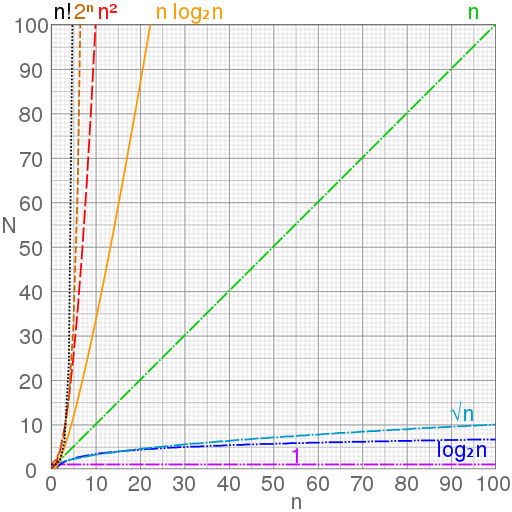
\includegraphics[width=9cm]{comp3.png} \\
Genauso sollte dadurch erkenntlich sein dass $n^{log_23}$ nicht in der selben Komplexitätsklasse ($\Theta$-mäßig zumindest) liegt wie $n^2$.
Oder dass (wenn man weiter raus-zoomen könnte würde das einfacher deutlich werden) $n^2$ und $2^n$ nicht in derselben liegen könnten.
% \lim_{n \mapsto \infty}{\frac{n * 1/n + log_2n}{log_23*n^{log_23 - 1}}} = \lim_{n \mapsto \infty}{\frac{\frac{1}{n*log_2n}}{}}$$.

% TODO: make right.

\section*{Aufgabe 3}
Der erste Programmcode quadriert eine Zahl auf sehr komische Art und Weise. Effektiv wäre es $\frac12*n^2$, allerdings ist
eben $\Theta(n^2)$ die einfachste Klasse in der es enthalten ist. \\ \\

Die Funktion \verb!id! gibt wieder die eingegebene Zahl zurück, aber tut das erst nach Laufzeit $3n$, fällt also erstmal in die
nichtmal an sich Böse Komplexitätsklasse $\Theta(n)$. \\ \\

\verb!rev! wiederum liefert eine Liste mit den Werten von der eingegebenen Zahl bis zur 1, in absteigender Reihenfolge. Aber nicht ohne erst
$n + \frac12 * n^2$ Operationen zu benötigen, wodurch wir wieder bei $\Theta(n^2)$ wären.


\subsection*{Placebo-Effekt}
Der Placebo-Effekt ist mehr als nur einbildung, es ist gewissermaßen eine Selbsterfüllende Prophezeihung, oder aus anderer Sicht ein
Mittel das dem Körper und Geist hilft, sich selbst zu helfen.

\end{document}

